\documentclass[10 pt,usenames,dvipsnames, oneside]{article}
\usepackage{../../modelo-fracoes}
\graphicspath{{../../../Figuras/licao04/}}


\begin{document}

\begin{center}
  \begin{minipage}[l]{3cm}

\includegraphics[width=2cm]{../../../Figuras/logo}       
\end{minipage}\hfill
\begin{minipage}[r]{.8\textwidth}
 {\Large \scshape Atividade: Retângulo maior com retângulos menores}  
\end{minipage}
\end{center}
\vspace{.2cm}

\ifdefined\prof
%Caixa do Para o Professor
\begin{goals}
%Objetivos específicos
\begin{enumerate}
\item       Reconhecer que as frações       $\frac{3}{10}$,
$\frac{6}{20}$, $\frac{9}{30}$, $\frac{18}{60}$ e $\frac{24}{80}$ são
iguais a partir da observação das representações destas frações em modelos de
área retangulares e dobraduras.
\end{enumerate}

\tcblower

%Orientações e sugestões
\begin{itemize}
\item       Recomenda-se que a atividade seja desenvolvida em grupos de 3 a
5 alunos e que, neste caso, cada grupo receba uma quantidade suficiente de
cópias das             folhas para reprodução. Podem ser necessárias mais
do que uma dessas folhas por aluno. Uma vez que a folha já tenha sido dobrada
para a realização de um dos itens, a marca deixada pode atrapalhar a realização
do item seguinte.
\item       É importante deixar claro para os alunos que, para decidir sobre
a quantidade de retângulos pintados e a quantidade total de retângulos menores, se devem considerar as divisões feitas pelos vincos das dobras. Neste sentido, você pode,
junto com a turma, a título de exemplo e de orientação, preencher a segunda
linha da tabela, deixando as demais para sejam preenchidas pelos grupos.
\item       É importante, ao final da atividade, observar para os alunos que
uma mesma parte do retângulo (a área da região pintada de amarelo) está sendo
descrita por frações com numeradores e denominadores diferentes (isto é, por
frações equivalentes), mas que, não obstante, por expressarem uma mesma
quantidade, estas frações são iguais.
\end{itemize}
\end{goals}

\bigskip
\begin{center}
{\large \scshape Atividade}
\end{center}
\fi

O \textit{retângulo maior} na folha que você recebeu está dividido em 10 retângulos menores, três deles estão coloridos. Dobre a folha como ilustrado na primeira coluna - ``Como dobrar''. As dobras formam novos \textit{retângulos menores}. Preencha a tabela a seguir, uma linha de cada vez, considerando as dobras feitas.
\begin{longtable}{|m{.30\textwidth}|m{.16\textwidth}|m{.16\textwidth}|m{.31\textwidth}|}
\hline
Como dobrar  &  Quantidade total de retângulos menores & Quantidade de retângulos menores pintados  &   Fração do retângulo maior do encarte que está pintada  \\
\hline \hline
\endhead
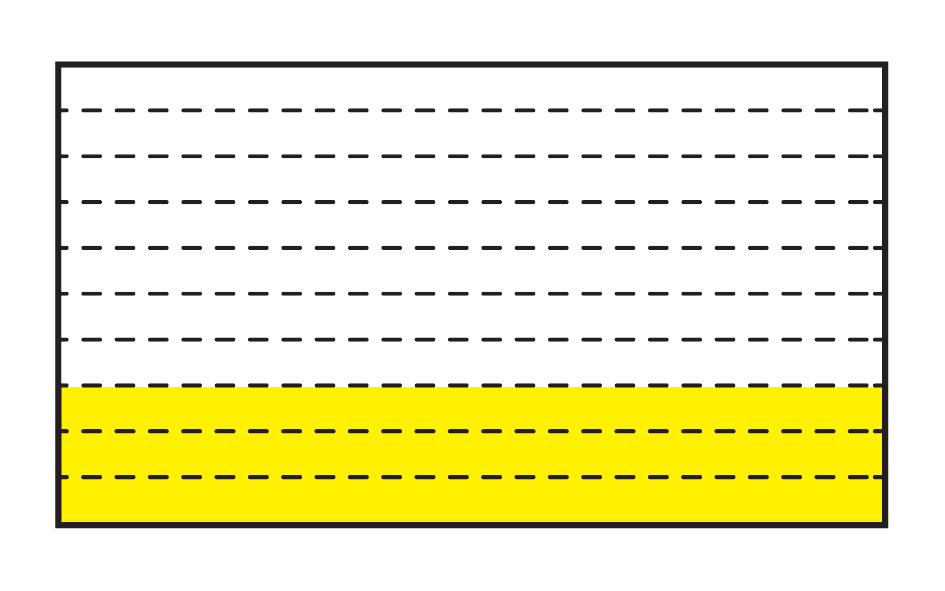
\includegraphics[width=100pt, keepaspectratio]{ativ2_fig01.png}      & $$10$$ & $$3$$&  $$\dfrac{3}{10}$$   \\
\hline
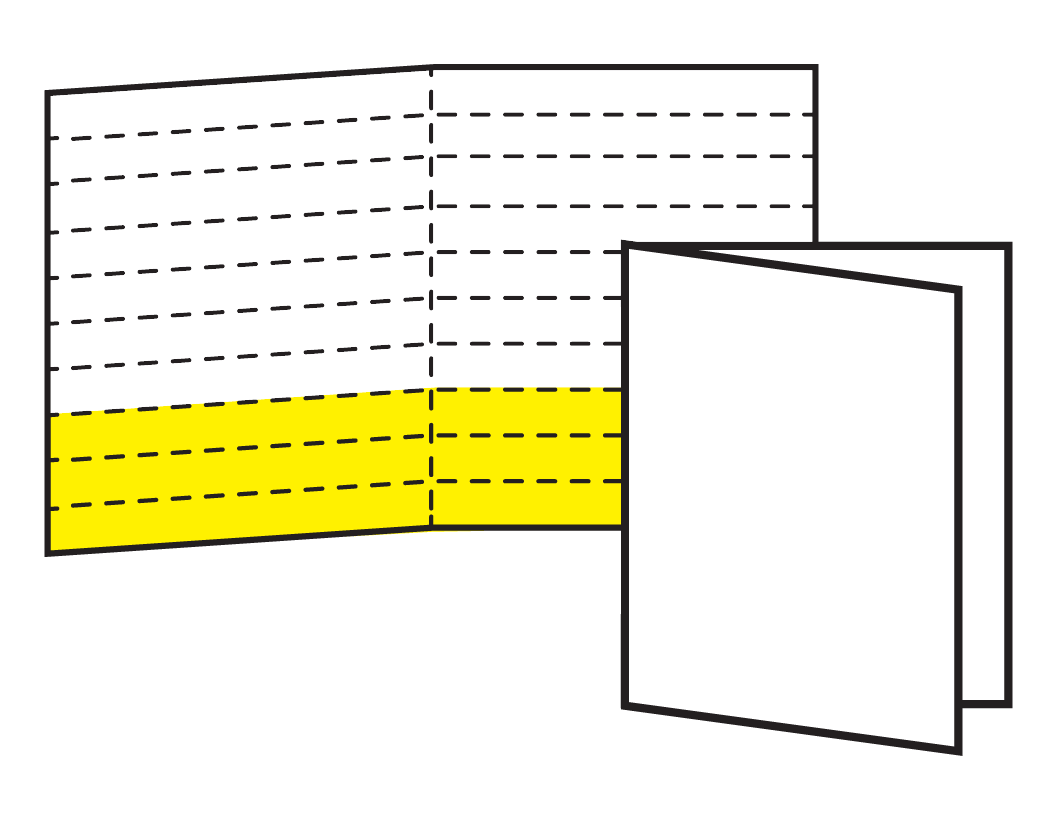
\includegraphics[width=100pt, keepaspectratio]{ativ2_fig02.png}                                                                              & &  &  \\
\hline
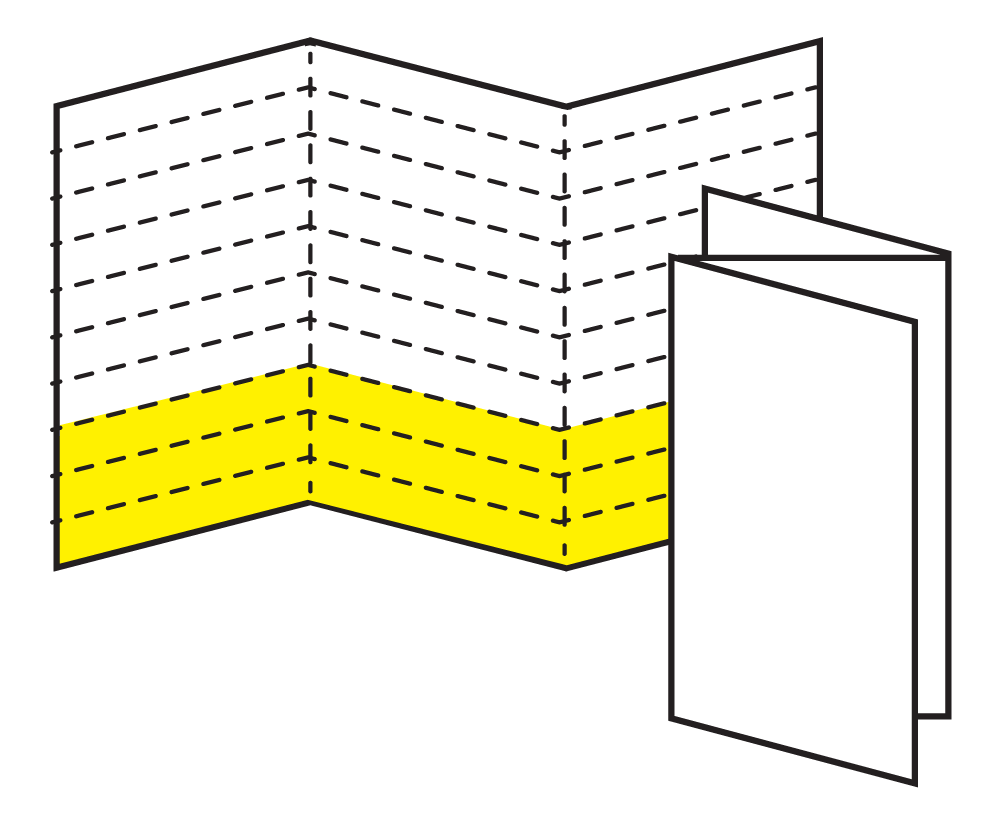
\includegraphics[width=100pt, keepaspectratio]{ativ2_fig03.png}     &  &   &  \\
\hline
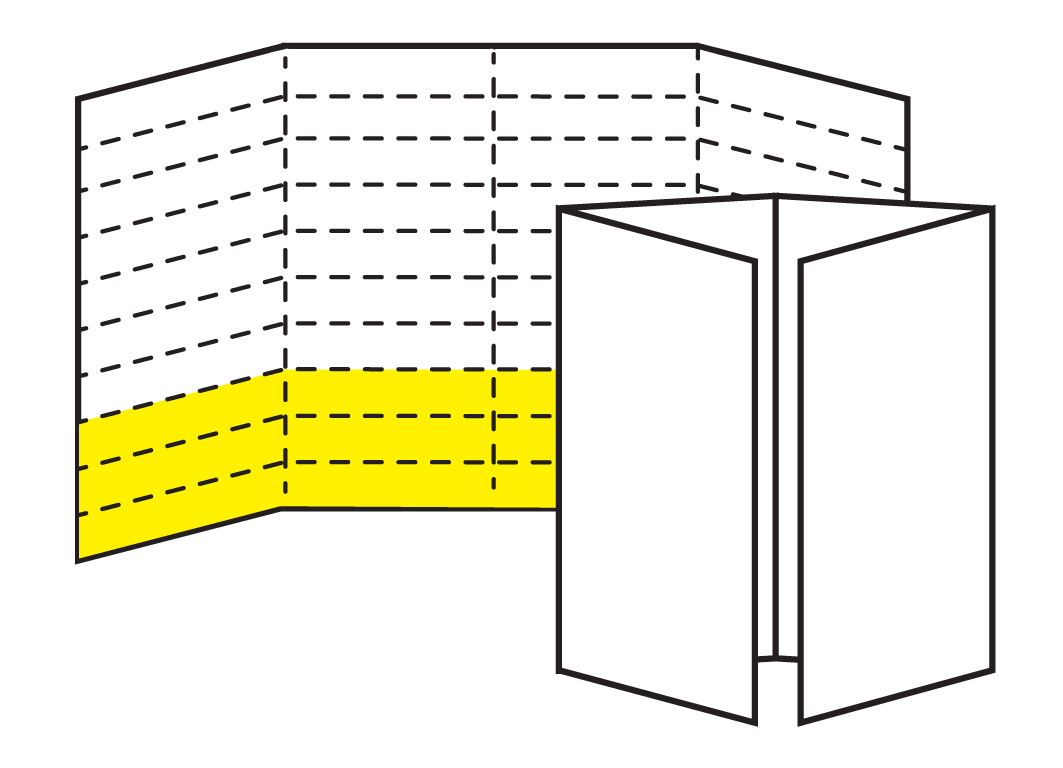
\includegraphics[width=100pt, keepaspectratio]{ativ2_fig04.png} & &&\\
\hline
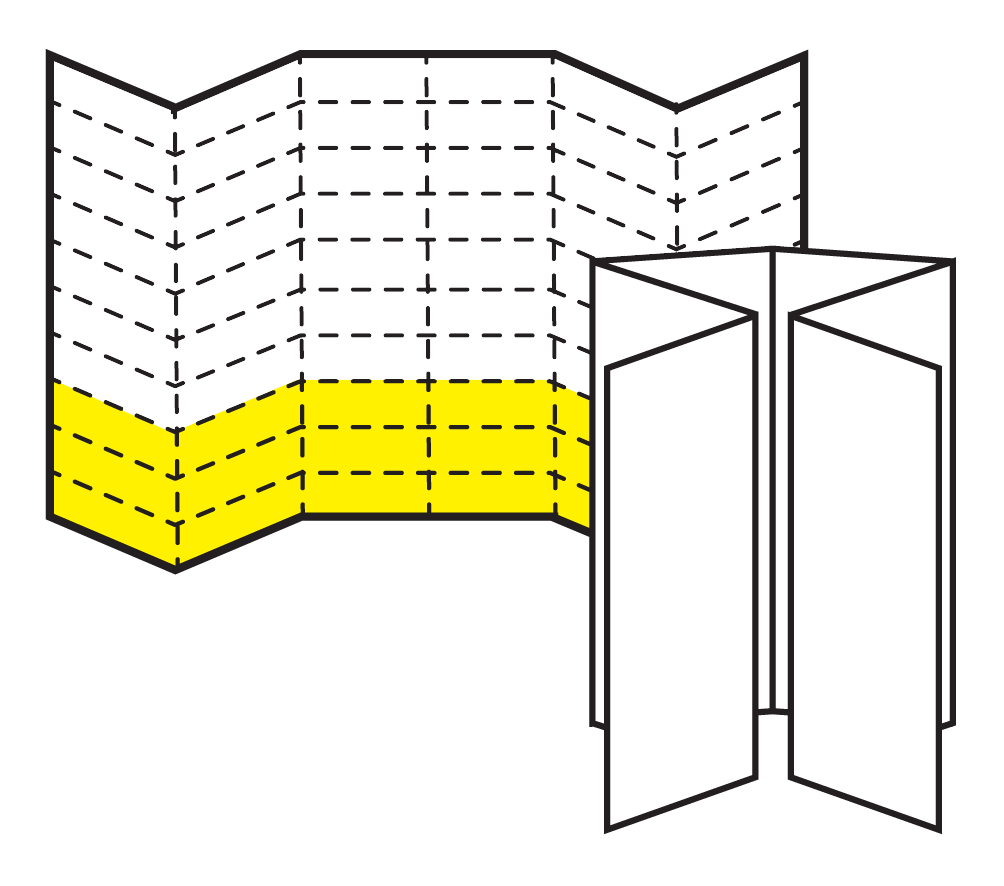
\includegraphics[width=100pt, keepaspectratio]{ativ2_fig05.png}  &                                     &                                  &                                                   \\
\hline
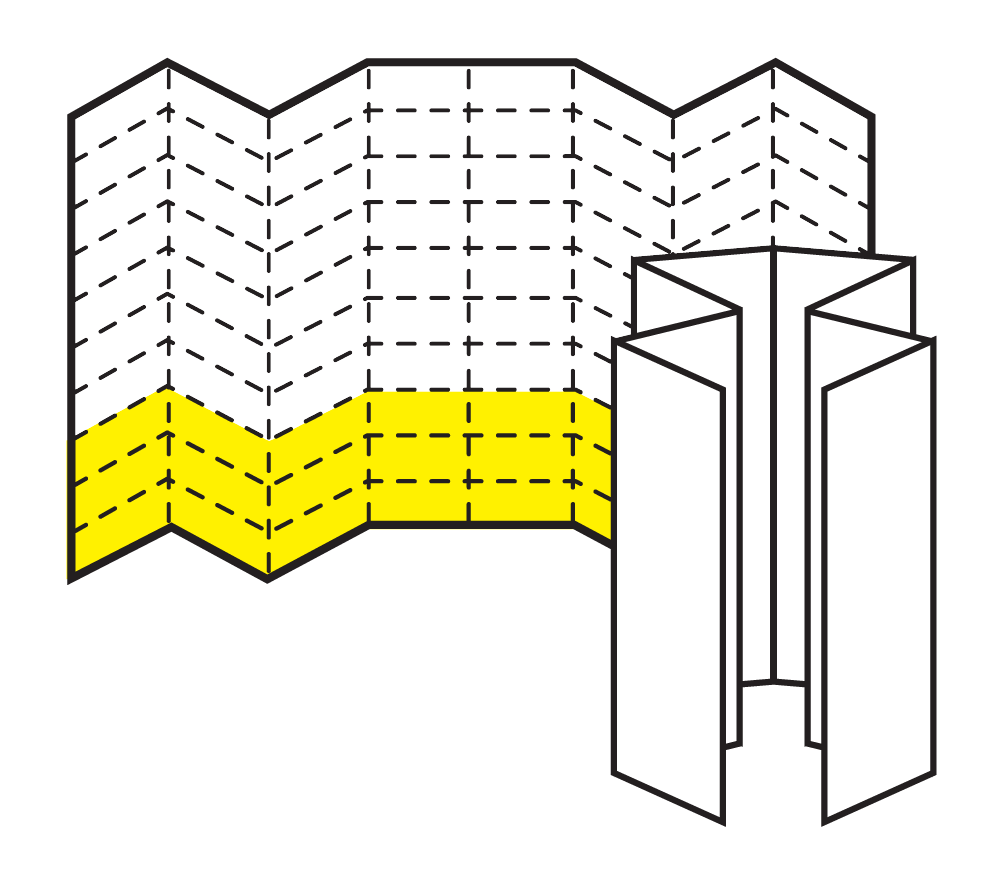
\includegraphics[width=100pt, keepaspectratio]{ativ2_fig06.png} &                                     &                                  &                                                   \\
\hline
\end{longtable}

\ifdefined\prof
\clearpage
\begin{solucao}
\vspace{1em}

\begin{tabular}{|m{.3\textwidth}|m{.16\textwidth}|m{.16\textwidth}|m{.21\textwidth}|}
\hline
Como dobrar  & Quantidade total de retângulos menores &  Quantidade de retângulos menores pintados   &  Fração do retângulo do encarte que está pintada  \\
\hline 
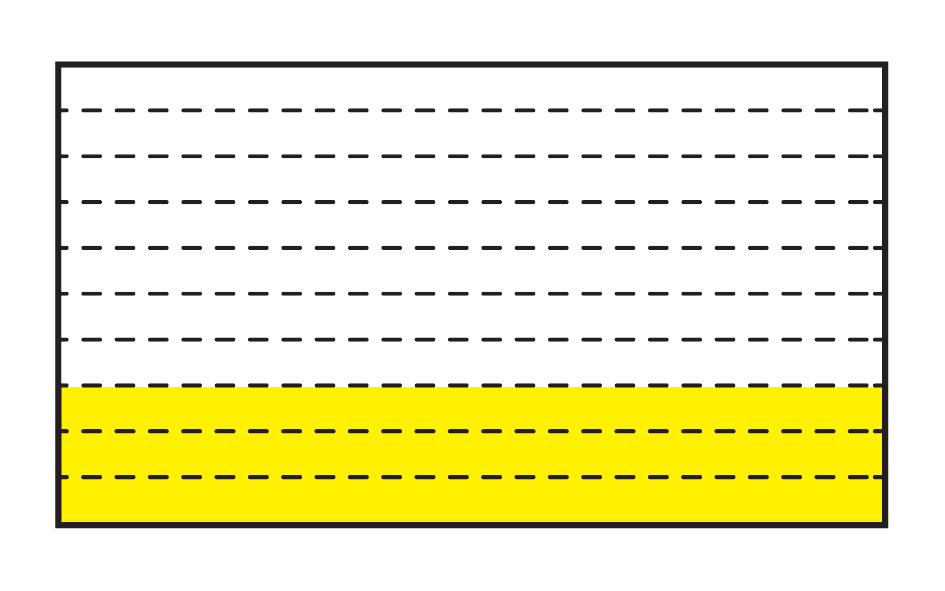
\includegraphics[width=100pt,
keepaspectratio]{ativ2_fig01.png} & 10 & 3 &  
$\frac{3}{10}$ \\
\hline
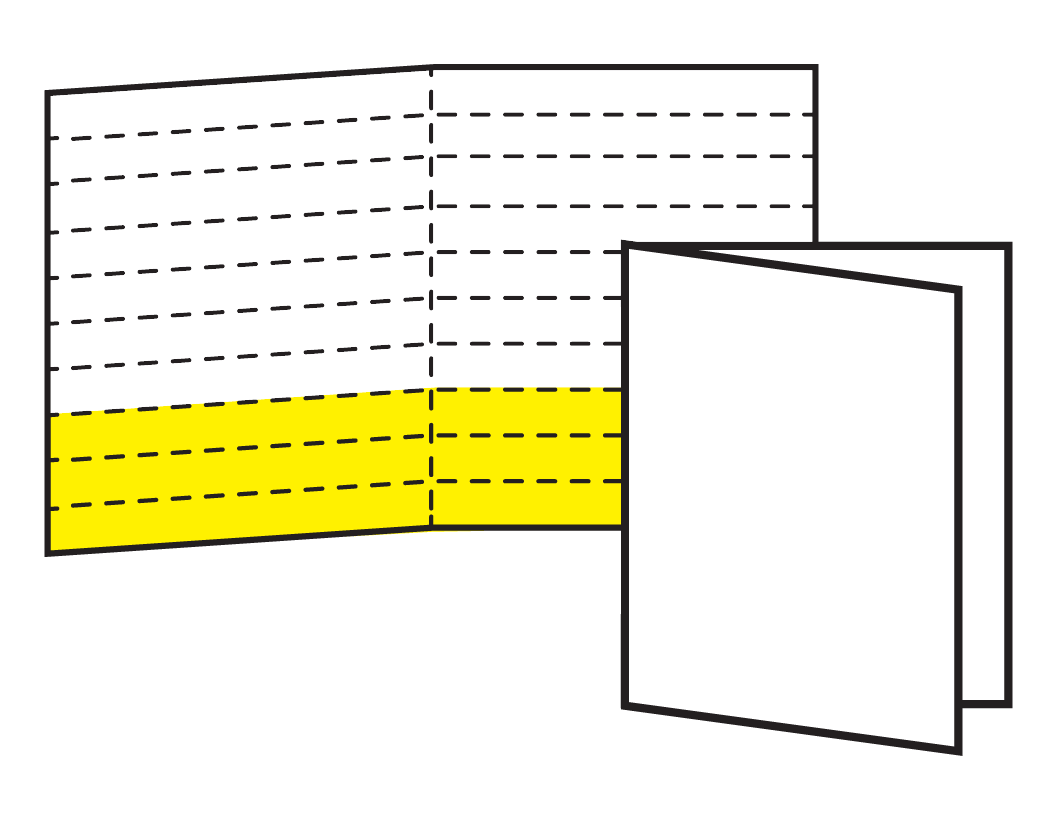
\includegraphics[width=100pt,
keepaspectratio]{ativ2_fig02.png} &  20 & 6 & 
$\frac{6}{20}$ \\
\hline
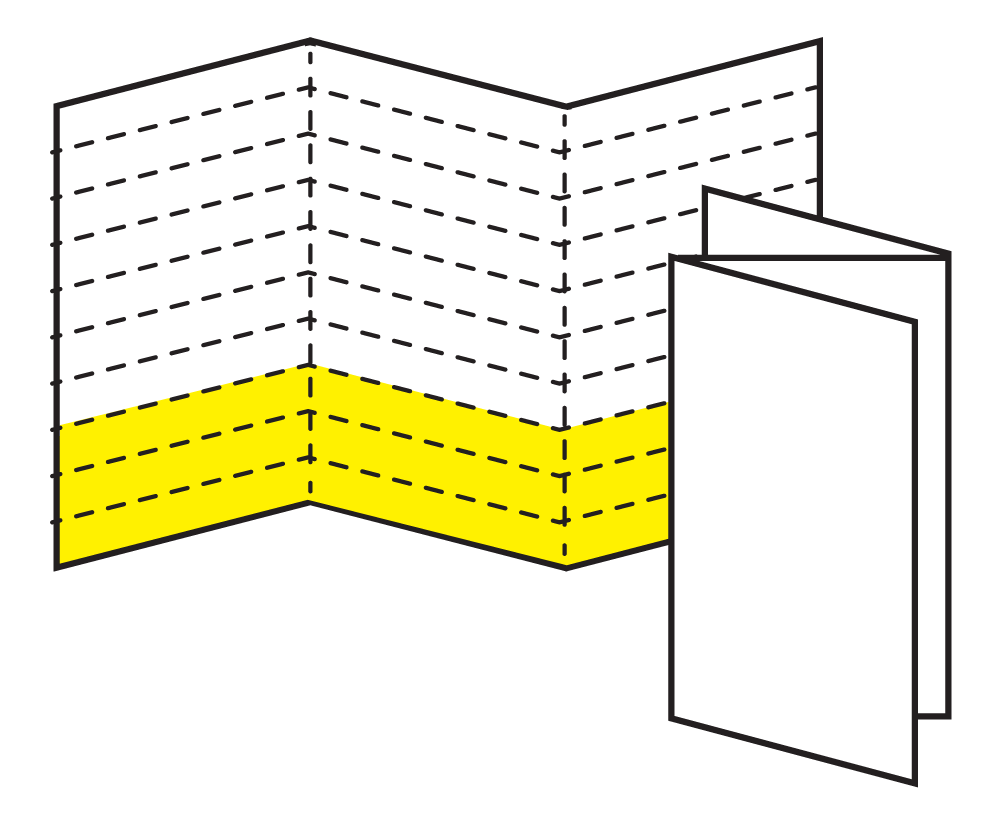
\includegraphics[width=100pt,
keepaspectratio]{ativ2_fig03.png} &  30 & 9 & 
$\frac{9}{30}$ \\
\hline
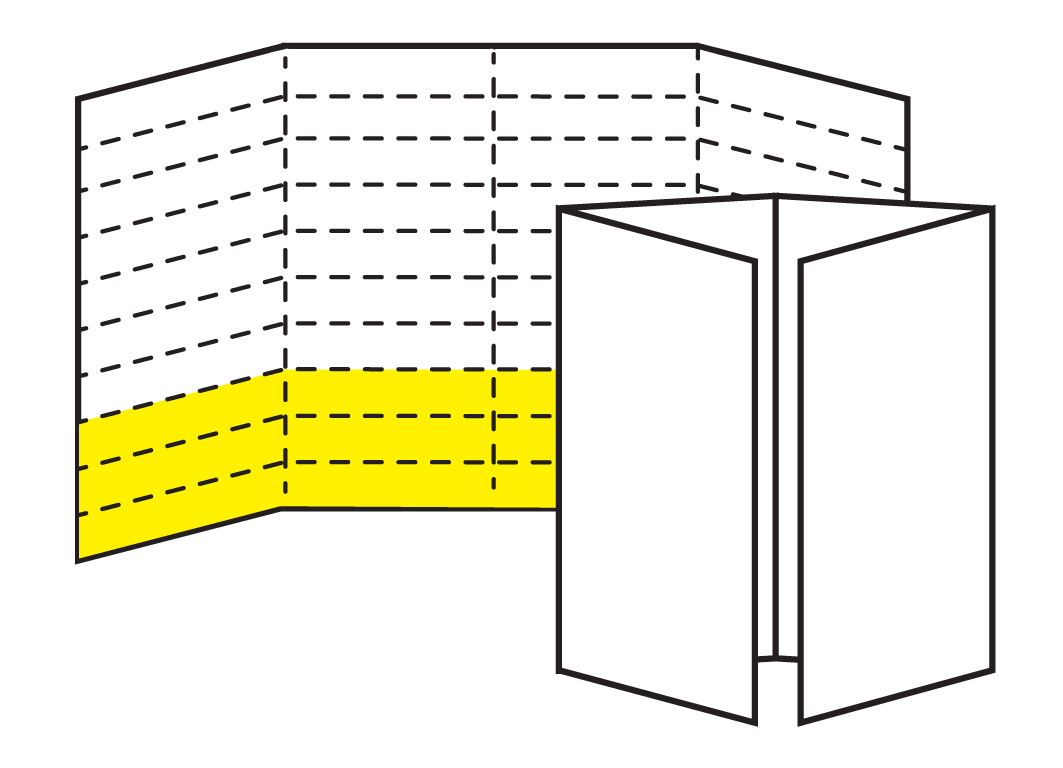
\includegraphics[width=100pt,
keepaspectratio]{ativ2_fig04.png} &  40 & 12 & 
$\frac{12}{40}$ \\
\hline
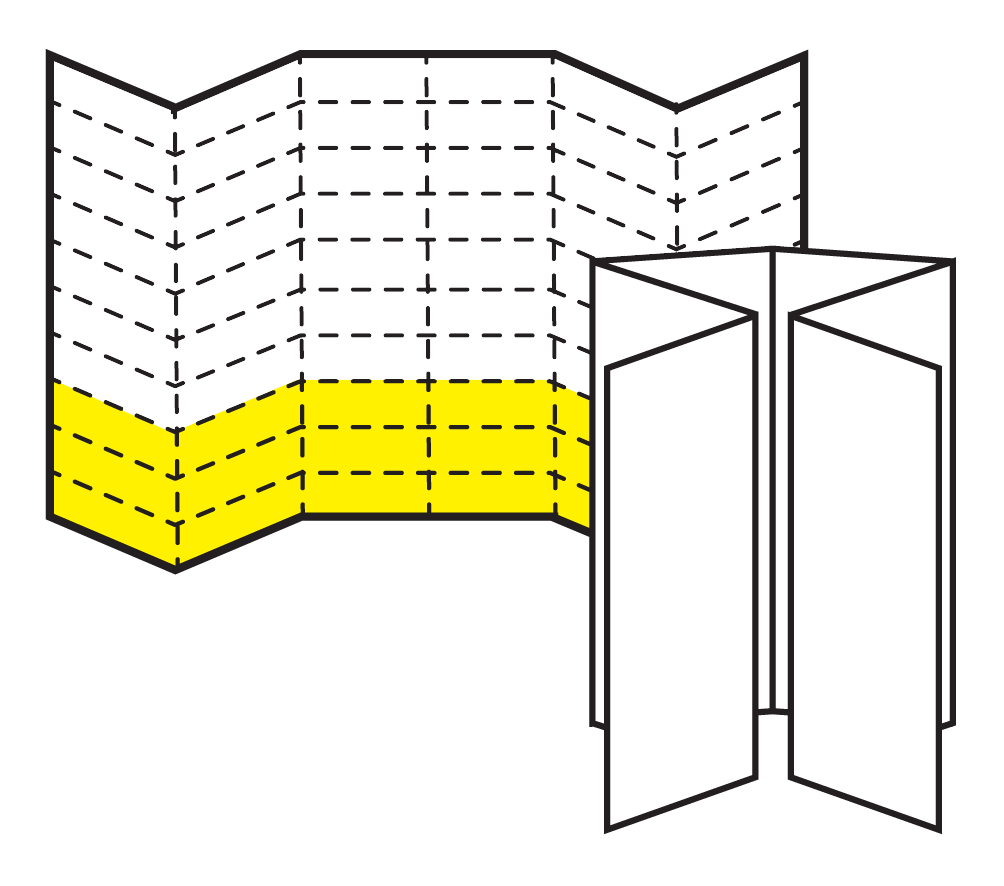
\includegraphics[width=100pt, keepaspectratio]{ativ2_fig05.png}&  60 & 18 &   $\frac{18}{60}$ \\
\hline
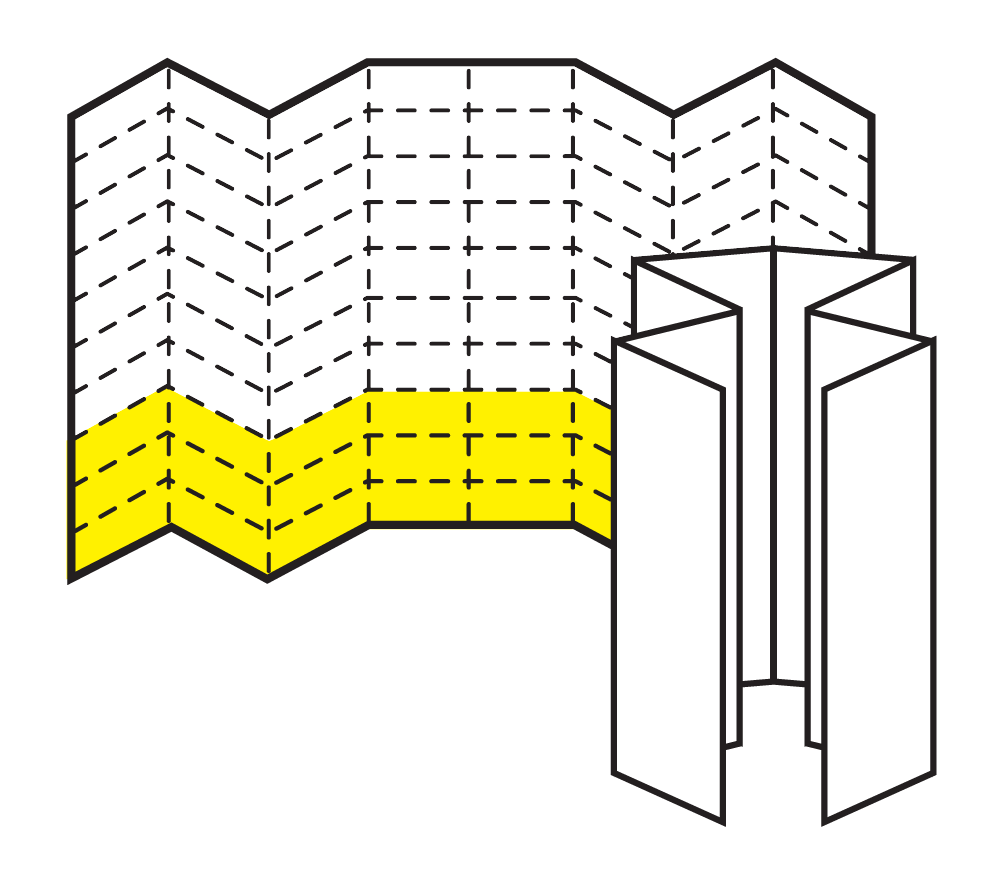
\includegraphics[width=100pt, keepaspectratio]{ativ2_fig06.png}&  80 & 24 &  $\frac{24}{80}$ \\
\hline
\end{tabular}

\end{solucao}
\fi

\end{document}